\documentclass{beamer}
\beamertemplatenavigationsymbolsempty
\usecolortheme{beaver}
\setbeamertemplate{blocks}[rounded=true, shadow=true]
\setbeamertemplate{footline}[page number]
%
\usepackage[utf8]{inputenc}
\usepackage[english, russian]{babel}
\usepackage{amssymb,amsfonts,amsmath,mathtext}
\usepackage{multirow}
\usepackage{graphicx} % Для масштабирования
\usepackage{subfig}
\usepackage{booktabs}
\usepackage[all]{xy} % xy package for diagrams
\usepackage{array}
\usepackage{multicol}% many columns in slide
\usepackage{hyperref}% urls
\usepackage{hhline}%tables
% Your figures are here:
\graphicspath{ {fig/} {../fig/} }

%----------------------------------------------------------------------------------------------------------
\title[\hbox to 56mm{Генерация}]{Accelerated Linearized Laplace Approximation for Bayesian Deep Learning}
\author[N.\,P.~Ivkin]{Stepanov Ilya}
\institute{Moscow Institute of Physics and Technology}
\date{\footnotesize
\par\bigskip\small 2025}

%----------------------------------------------------------------------------------------------------------
\begin{document}
%----------------------------------------------------------------------------------------------------------
\begin{frame}
\thispagestyle{empty}
\maketitle
\end{frame}
%-----------------------------------------------------------------------------------------------------

%------------------------------------------------------------------------------------------

\begin{frame}{Bayesian Neural Networks: Basic Concepts}

\begin{block}{Problem with Neural Networks}
\begin{itemize}
\item Neural networks $g_\theta(x)$ find only the \textbf{most probable} interpretation of data
\item \textbf{Do not account for uncertainty}: prone to overfitting and overconfidence
\end{itemize}
\end{block}

\begin{block}{Solution: Bayesian Approach}
\begin{itemize}
\item Introduce \textbf{prior distribution} $p(\theta)$ on parameters
\item Seek \textbf{posterior distribution}: 
$$p(\theta|D) = \frac{p(D|\theta)p(\theta)}{p(D)}$$
\item Analytically intractable due to neural network nonlinearity
\end{itemize}
\end{block}

\end{frame}

\begin{frame}{Inference and Prediction in BNN}

\begin{block}{Approximate Inference Methods}
Find approximation $q(\theta) \approx p(\theta|D)$:
\begin{itemize}
\item Variational Inference (VI)
\item Laplace Approximation (LA)
\item MCMC methods
\item POVI
\end{itemize}
\end{block}

\begin{block}{BNN Prediction}
For new $x^*$ prediction:
$$p(y|x^*,D) = \mathbb{E}_{p(\theta|D)}p(y|x^*,\theta) \approx \mathbb{E}_{q(\theta)}p(y|x^*,\theta) \approx \frac{1}{S}\sum_{s=1}^S p(y|g_{\theta_s}(x^*))$$
where $\theta_s \sim q(\theta)$ - parameter samples
\end{block}

\end{frame}


\begin{frame}{Laplace Approximation (LA)}

\begin{block}{Laplace Approximation (LA)}
Builds Gaussian approximate posterior:
$$q(\theta) = \mathcal{N}(\theta; \hat{\theta}, \Sigma)$$
where:
\begin{itemize}
\item $\hat{\theta} = \arg\max_\theta (\log p(D|\theta) + \log p(\theta))$ (MAP estimate)
\item $\Sigma^{-1} = -\nabla^2_{\theta\theta} (\log p(D|\theta) + \log p(\theta))|_{\theta=\hat{\theta}}$ (Hessian)
\end{itemize}
\end{block}

\begin{block}{With Gaussian Prior}
For $p(\theta) = \mathcal{N}(\theta; 0, \sigma_0^2 I_P)$:
$$-\nabla^2_{\theta\theta} \log p(\theta)|_{\theta=\hat{\theta}} = I_P / \sigma_0^2$$
\end{block}

\end{frame}

\begin{frame}{Generalized Gauss-Newton (GGN) Approximation}

\begin{block}{GGN Approximation}
Due to Hessian intractability:
$$\Sigma^{-1} = \sum_{i=1}^N J_{\hat{\theta}}(x_i)^\top \Lambda(x_i,y_i) J_{\hat{\theta}}(x_i) + I_P / \sigma_0^2$$
where:
\begin{itemize}
\item $J_{\hat{\theta}}(x) = \nabla_\theta g_\theta(x)|_{\theta=\hat{\theta}}$ (Jacobian)
\item $\Lambda(x, y) = -\nabla^2_{gg} \log p(y|g)|_{g=g_{\hat{\theta}}(x)}$ (Likelihood Hessian)
\end{itemize}
\end{block}

\end{frame}

\begin{frame}{Scalability Issues}

\begin{block}{Scalability Challenges}
The GGN (Generalized Gauss–Newton) matrix of size $P \times P$ is intractable for large networks.
\end{block}

\begin{itemize}
    \item \textbf{Diagonal approximation}: keeps only diagonal elements
    \item \textbf{KFAC approximation}: block-diagonal structure via Kronecker factorization
    \item \textbf{Subspace methods}: reduce dimensionality (e.g., last layer only)
\end{itemize}

\vspace{0.3cm}

\end{frame}

\begin{frame}{Linearized Laplace Approximation (LLA)}

\begin{block}{Idea}
To align prediction, use a linearized model:
\[
g_\theta^{\text{lin}}(x) = g_{\hat{\theta}}(x) + J_{\hat{\theta}}(x)(\theta - \hat{\theta})
\]
\end{block}

\begin{block}{Approximating Distributions}
\begin{itemize}
    \item \textbf{Parameter posterior}: $p(\theta|D) \approx \mathcal{N}(\theta; \hat{\theta}, \Sigma)$
    \item \textbf{Likelihood}: $p(y^*|\theta, x^*) \approx \mathcal{N}(y^*; g_{\hat{\theta}}(x^*) + J_{\hat{\theta}}(x^*)(\theta - \hat{\theta}), \sigma_1^2)$
\end{itemize}
\end{block}

\begin{block}{Bayesian Predictive Distribution}
Using linear-Gaussian model properties:
\[
p(y^*|x^*, D) \approx \mathcal{N}\left(y^*; g_{\hat{\theta}}(x^*), \sigma_1^2 + J_{\hat{\theta}}(x^*) \Sigma J_{\hat{\theta}}(x^*)^T\right)
\]
\end{block}

\end{frame}

% --- SLIDE 1 ---
\begin{frame}{Gaussian Process View of LLA}

\begin{block}{From Parameter Space to Function Space}
We move from a parameter-space view to a
\textbf{function-space Gaussian process (GP)}:
$$
q(f) = \mathrm{GP}\big(f \mid g_{\hat{\theta}}(x), \kappa_{\text{LLA}}(x, x')\big)
$$
with kernel
$$
\kappa_{\text{LLA}}(x, x') = J_{\hat{\theta}}(x)\Sigma J_{\hat{\theta}}(x')^\top
$$
\end{block}

\begin{itemize}
    \item LLA represents a neural network as a Gaussian Process around its MAP estimate.
\end{itemize}

\end{frame}


% --- SLIDE 2 ---
\begin{frame}{Neural Tangent Kernel}

\begin{block}{Connection to Neural Tangent Kernel (NTK)}
Using the Woodbury identity, the covariance matrix can be rewritten as:
$$
\Sigma = \sigma_0 I_P - J_{\hat{\theta}, X}
\Big[
\Lambda_{X,Y}/\sigma_0 + J_{\hat{\theta}, X}J_{\hat{\theta}, X}^\top
\Big]^{-1}
J_{\hat{\theta}, X}^\top
$$

Substituting into $\kappa_{\text{LLA}}$ yields:
\begin{align*}
\kappa_{\text{LLA}}(x, x')
&= \sigma_0^2 \Big[
      \kappa_{\text{NTK}}(x, x')
      - 
      \kappa_{\text{NTK}}(x, X)
      \Big(
          \Lambda_{X,Y}^{-1}/\sigma_0^2 
          + \kappa_{\text{NTK}}(X, X)
      \Big)^{-1} \\
&\quad \cdot 
      \kappa_{\text{NTK}}(X, x')
   \Big]
\end{align*}



where
$$
\kappa_{\text{NTK}}(x, x') = J_{\hat{\theta}}(x)J_{\hat{\theta}}(x')^\top
$$

\end{block}


\end{frame}



\begin{frame}{Scalability Limitations of LLA}

\begin{block}{Main Bottleneck}
Computing and inverting the matrix
$$
\kappa_{\text{NTK}}(X, X) \in \mathbb{R}^{(N \cdot C) \times (N \cdot C)}
$$
is computationally infeasible when $N$ or $C$ is large.
\end{block}

\vspace{0.3cm}

\textbf{→ Solution: Accelerated kernel Approximation for LLA (ELLA).}

\end{frame}

\begin{frame}{Nyström Approximation for NTK}

\begin{block}{Main Idea}
We approximate the NTK using a low-rank feature map:
\[
\kappa_{\text{NTK}}(x, x') \approx \phi(x)\phi(x')^\top,
\]
where $\phi: \mathcal{X} \to \mathbb{R}^{C \times K}$ captures the top-$K$ spectral components of the NTK.
\end{block}

\begin{itemize}
    \item Select $M$ landmark pairs $\widetilde{X} = \{(x_m, i_m)\}_{m=1}^M$.
    \item Compute matrix 
    \[
        K = J_{\hat{\theta}, \widetilde{X}} J_{\hat{\theta}, \widetilde{X}}^\top
    \]
      from Jacobians of selected points.
    \item Obtain top-$K$ eigenpairs $(\lambda_k, u_k)$ of $K$.
    \item Define feature map:
    \[
        \phi(x) = [J_{\hat{\theta}}(x)v_1, \dots, J_{\hat{\theta}}(x)v_K], 
        \quad v_k = \frac{J_{\hat{\theta}, \widetilde{X}}^\top u_k}{\sqrt{\lambda_k}}.
    \]
\end{itemize}

\end{frame}


\begin{frame}{Accelerating LLA via Kernel Approximation (ELLA)}

% \begin{block}{Kernel Approximation Idea}
% If NTK can be approximated as an inner product:
% $$
% \kappa_{\text{NTK}}(x, x') \approx \phi(x)\phi(x')^\top,
% $$
% with $\phi : \mathcal{X} \to \mathbb{R}^{C \times K}$, then scalability improves drastically.
% \end{block}

% \begin{itemize}
%     \item Define $\phi_X = [\phi(x_1), \dots, \phi(x_N)]^\top \in \mathbb{R}^{NC \times K}$.
%     \item Approximate LLA kernel:
%     $$
%     \kappa_{\text{ELLA}}(x, x') = \phi(x) \left[
%     \sum_i \phi(x_i)^\top \Lambda_{x_i,y_i}\phi(x_i) + \frac{I_K}{\sigma_0^2}
%     \right]^{-1} \phi(x')^\top
%     $$
%     \item Small $K$ (e.g. $<100$) makes inversion cheap.
% \end{itemize}


% \end{frame}
% % ---------------- Slide: Nyström intuition ----------------
% % ---------------- Slide: Nyström approximation (intuition + idea) ---------------


% % ---------------- Slide: ELLA with Nyström features ----------------
% \begin{frame}{ELLA: Efficient Linearized Laplace Approximation}

\begin{block}{Compact kernel form}
Using $\phi(x)$, we approximate the predictive covariance of LLA:
\[
\kappa_{\text{ELLA}}(x, x') = 
\phi(x)
\left[
\sum_i \phi(x_i)^\top \Lambda(x_i, y_i)\phi(x_i)
+ \frac{I_K}{\sigma_0^2}
\right]^{-1}
\phi(x')^\top
\]
\end{block}

\begin{itemize}
    \item Reduces $P\times P$ inversion to $K\times K$ (\(K \ll P\)).
    \item Preserves the GP interpretation of LLA.
    \item Enables fast uncertainty estimation with pretrained networks.
    \item Empirically stable for $K<100$.
\end{itemize}

\end{frame}


% ---------------- Slide: Practical tips & trade-offs ----------------
\begin{frame}{ELLA Implementation Overview}


\begin{block}{Algorithm 1: Estimate Posterior $q(f)$}
\begin{itemize}
    \item Compute $G = \sum_i \phi(x_i)^\top \Lambda_{x_i, y_i}\phi(x_i) + I_K/\sigma_0^2$.
    \item Invert: $G^{-1}$.
    \item Posterior predictive $q(f(x)) = \mathcal{N}(g_{\hat{\theta}}(x), \phi(x)G^{-1}\phi(x)^\top)$
\end{itemize}
\end{block}

\begin{block}{Algorithm 2: Build Feature Map $\phi$ (Nyström Approximation)}
\begin{itemize}
    \item Select $M$ random landmark pairs $(x_m, i_m)$.
    \item Compute Jacobians $J_{\hat{\theta}, \widetilde{X}}[m] = \nabla_{\hat{\theta}} g_{\hat{\theta}}(x_m)[i_m]$.
    \item Perform eigendecomposition of $K = J_{\hat{\theta}, \widetilde{X}} J_{\hat{\theta}, \widetilde{X}}^\top$.
    \item Define $v_k = J_{\hat{\theta}, \widetilde{X}}^\top u_k / \sqrt{\lambda_k}$.
    \item Build $\phi(x) = [J_{\hat{\theta}}(x)v_1, \dots, J_{\hat{\theta}}(x)v_K]$.
\end{itemize}
\end{block}

\end{frame}




% {\small Определим датасет как $ \mathfrak{D}=\{ {x}_{i}: i = 1, \dots, n\}$, ${x}_{i}$ --- изображение. Рассматривается диффузионная модель для аугментации $\epsilon_{\theta}$. Определим функцию потерь:
% \begin{center}
%     $\mathcal{L}(\epsilon, \epsilon_{\theta}) = \mathbb{E}_{\epsilon \sim N(0, I), m_i, \tau_i, \tilde{x_i}, t} \|\epsilon - \epsilon_{\theta}(x^t_i, m_i,\tau_i, \tilde{x_i}, t)\|^2,$
% \end{center}
% где $x^t_i$ -- зашумленное изображение на шаге $t$, $m_i$ -- сегментационная маска данного изображения, $\tau_i$ -- текстовая подсказка данного изображения,
% $\tilde{x_i}$ = $(1 - m_i) \ \odot x_i$, $t \in [0, T]$ -- шаг диффузионного процесса. Для получения масок и текстовых подсказок мы используем модели сегментации и "image-to-text".
% % Модифицированный датасет после аугментаций определим как $\tilde{\mathfrak{D}} = \{ \phi_{\theta}({x}_{i}): i = 1, \dots, n\}$, ${x}_{i}$ --- изображение. Требуется оценить качество синтетических данных $\tilde{\mathfrak{D}}$, используя модели детекции.
% }

% {Рассмотрим генеративную аугментацию как соответствие:
% \begin{center}
%     $f_{\theta}: X \to Y,$
% \end{center}
% где:

% \begin{itemize}
%     \item $X=\{ x_{i}: i = 1, \dots, n\}$ — пространство входных изображений;
%     \item $Y=\{ y_{i}: i = 1, \dots, n\}$ — пространство аугментированных изображений;
%     \item $f_{\theta}$ — генеративная модель с параметрами $\theta$, преобразующая входное изображение $x_i$ в аугментированное изображение $y_i$.
% \end{itemize}



% }

%------------------------------------------------------------------------------------------

\begin{frame}{Experimental Results: Uncertainty in ELLA}

\begin{block}{Test accuracy and ECE on CIFAR-10}
\begin{figure}[h]
    \centering
    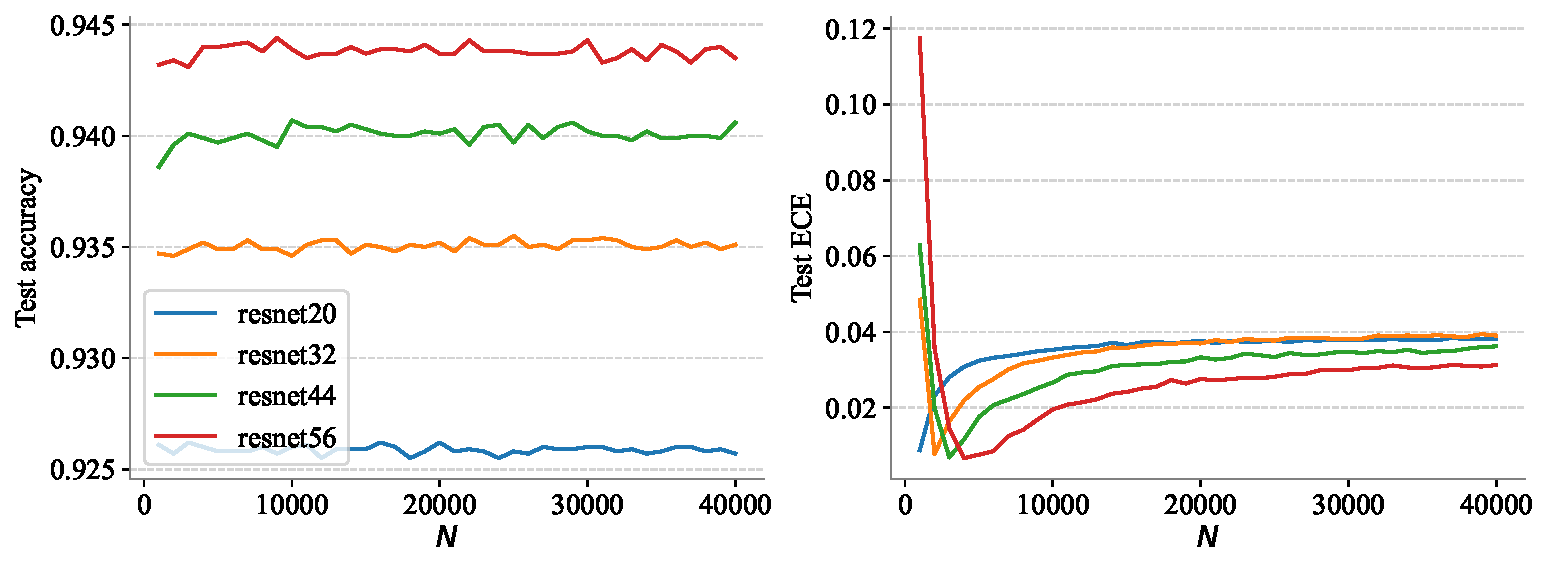
\includegraphics[width=0.8\textwidth]{test_curve.pdf}
    \caption{Test accuracy and ECE of ELLA vs. number of training samples N}
    \label{fig:nll}
\end{figure}

\footnotesize
\textsuperscript{*}Expected Calibration Error (ECE):
\[
\text{ECE} = \sum_{m=1}^M \frac{|B_m|}{n} \left|\text{acc}(B_m) - \text{conf}(B_m)\right|
\]
\scriptsize
$M$: bins, $n$: samples, $|B_m|$: bin size, $\text{acc}(B_m) = \frac{1}{|B_m|}\sum_{i \in B_m} \mathbb{I}(\hat{y}_i = y_i)$: bin accuracy, 
$\text{conf}(B_m) = \frac{1}{|B_m|}\sum_{i \in B_m} \hat{p}_i$: bin confidence
\end{block}

\end{frame}

\begin{frame}{Experimental Results: Uncertainty in ELLA}

\begin{block}{Test NLL on CIFAR-10}
\begin{figure}[h]
    \centering
    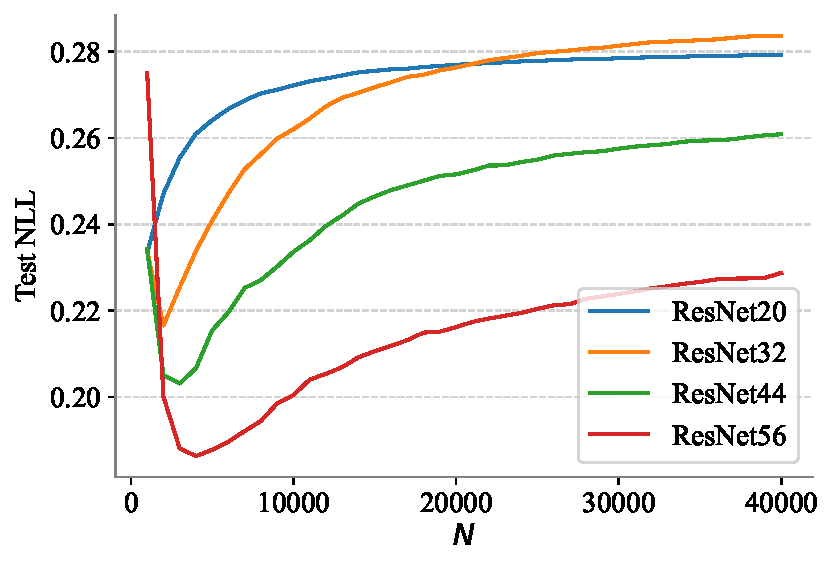
\includegraphics[width=0.8\textwidth]{test_curve2.pdf}
    \caption{Test NLL of ELLA vs. number of training samples N.}
    \label{fig:nll}
\end{figure}
\end{block}

\end{frame}

\begin{frame}{Experimental Results: Regression}

\begin{block}{Regression problem}
\begin{figure}[h]
    \centering
    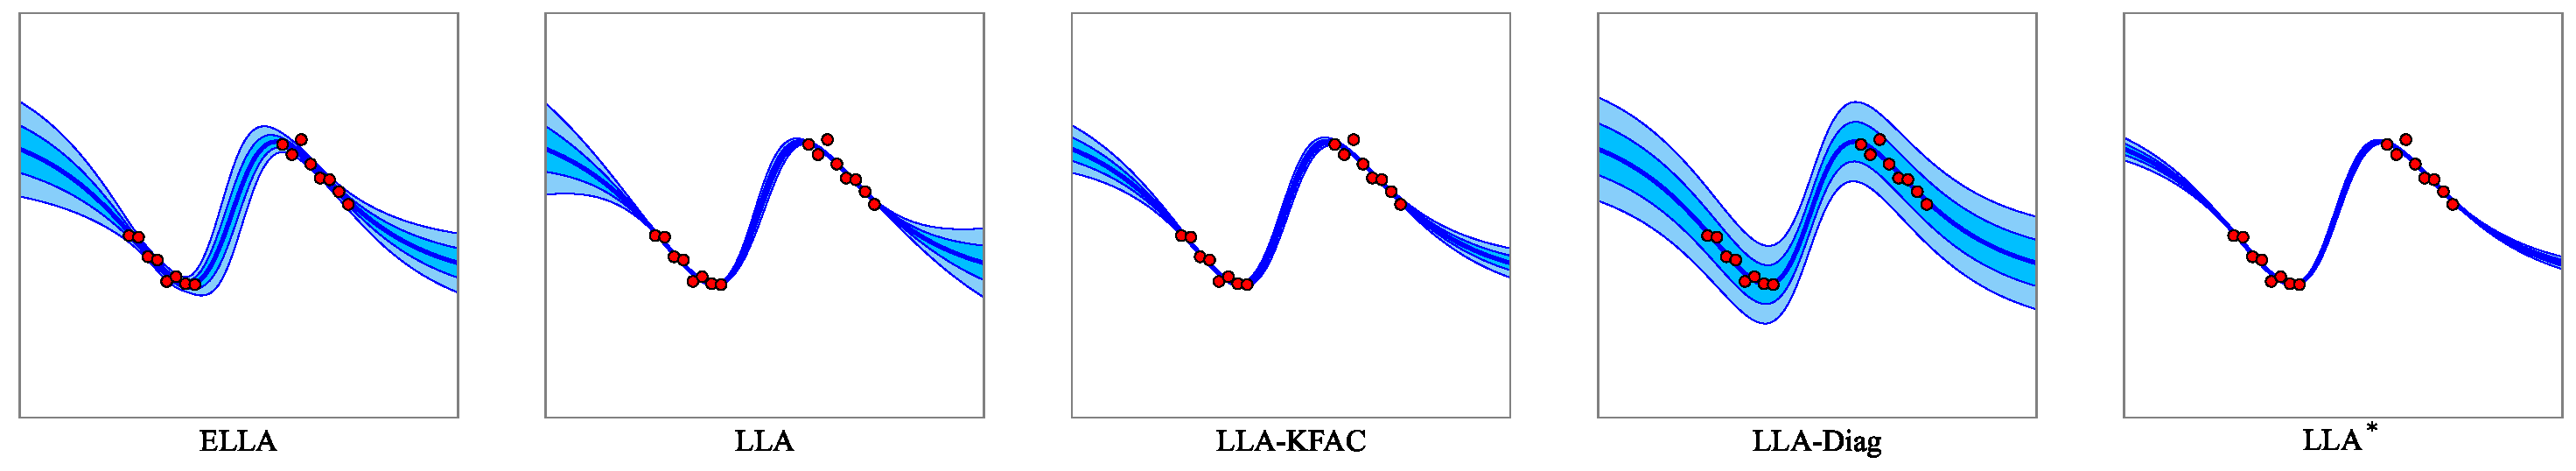
\includegraphics[width=1.0\textwidth]{toy_regression.pdf}
    \caption{Regression on $y = \sin(2x) + \varepsilon$, $\varepsilon \sim \mathcal{N}(0, 0.2)$. Red dots, central blue curves, and shaded regions refer to the training data, mean predictions, and uncertainty respectively. The model is a pretrained multilayer perceptron (MLP) with 3 hidden layers.}
    \label{fig:nll}
\end{figure}
\end{block}
\vspace{-0.9cm}
\begin{table}[h]
\centering
\caption{Comparison on the approximation error to vanilla LLA in the illustrative regression case, measured by the KL divergence between the predictive distributions.}
\begin{tabular}{lcccc}
\toprule
Method & ELLA & LLA-KFAC & LLA-Diag & LLA$_*$ \\
\midrule
KL div. & 0.83 & 0.35 & 1.71 & 2.44 \\
\bottomrule
\end{tabular}
\label{tab:comparison}
\end{table}


\end{frame}

\begin{frame}{Experimental Results: Classification}

\begin{table}[t]
  \centering
  \tiny
  \caption{Comparison on CIFAR-10 test accuracy (\%) $\uparrow$, NLL $\downarrow$, and ECE $\downarrow$. Average over 5 runs.}
  \vskip 0.05in
  \label{table:3}
  \setlength{\tabcolsep}{2.5pt}
  \begin{tabular}{lcccccccccccc}
  \toprule
  \multirow{2}{*}{Method} & \multicolumn{3}{c}{ResNet-20} & \multicolumn{3}{c}{ResNet-32} & \multicolumn{3}{c}{ResNet-44} & \multicolumn{3}{c}{ResNet-56} \\
  \cmidrule(lr){2-4} \cmidrule(lr){5-7} \cmidrule(lr){8-10} \cmidrule(l){11-13}
  & Acc & NLL & ECE & Acc & NLL & ECE & Acc & NLL & ECE & Acc & NLL & ECE \\
  \midrule
  
  \emph{ELLA}      & 92.5 & 0.233 & \textbf{0.009} & 93.5 & \textbf{0.215} & \textbf{0.008} & 93.9 & \textbf{0.204} & \textbf{0.007} & 94.4 & \textbf{0.187} & \textbf{0.007} \\
  \emph{MAP}       & 92.6 & 0.282 & 0.039 & 93.5 & 0.292 & 0.041 & 94.0 & 0.275 & 0.039 & 94.4 & 0.252 & 0.037 \\
  \emph{MFVI-BF}   & 92.7 & \textbf{0.231} & 0.016 & 93.5 & 0.222 & 0.020 & 93.9 & 0.206 & 0.018 & 94.4 & 0.188 & 0.016 \\
  \emph{LLA$^*$}   & 92.6 & 0.269 & 0.034 & 93.5 & 0.259 & 0.033 & 94.0 & 0.237 & 0.028 & 94.4 & 0.213 & 0.022 \\
  \emph{LLA$^*$-KFAC} & 92.6 & 0.271 & 0.035 & 93.5 & 0.260 & 0.033 & 94.0 & 0.232 & 0.028 & 94.4 & 0.202 & 0.024 \\
  \emph{LLA-Diag}  & 92.2 & 0.728 & 0.404 & 92.7 & 0.755 & 0.430 & 92.8 & 0.778 & 0.445 & 92.9 & 0.843 & 0.480 \\
  \emph{LLA-KFAC}  & 92.0 & 0.852 & 0.467 & 91.8 & 1.027 & 0.547 & 91.4 & 1.091 & 0.566 & 89.8 & 1.174 & 0.579 \\
  \bottomrule
  \end{tabular}
\end{table}


\end{frame}

\begin{frame}{Experimental Results: Classification}

\begin{figure}[h]
    \centering
    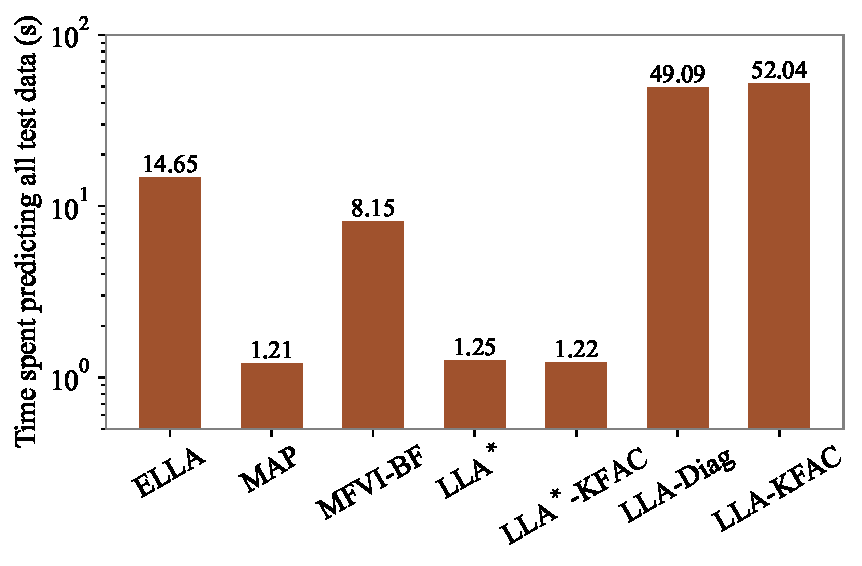
\includegraphics[width=0.4\textwidth]{time_comp.pdf}
    \caption{Comparison on the wall-clock time used for predicting all CIFAR-10 test data (measured on an NVIDIA A40 GPU) with ResNet-20.}
    \label{fig:time}
\end{figure}

\begin{columns}
\begin{column}{0.5\textwidth}
\begin{figure}[h]
    \centering
    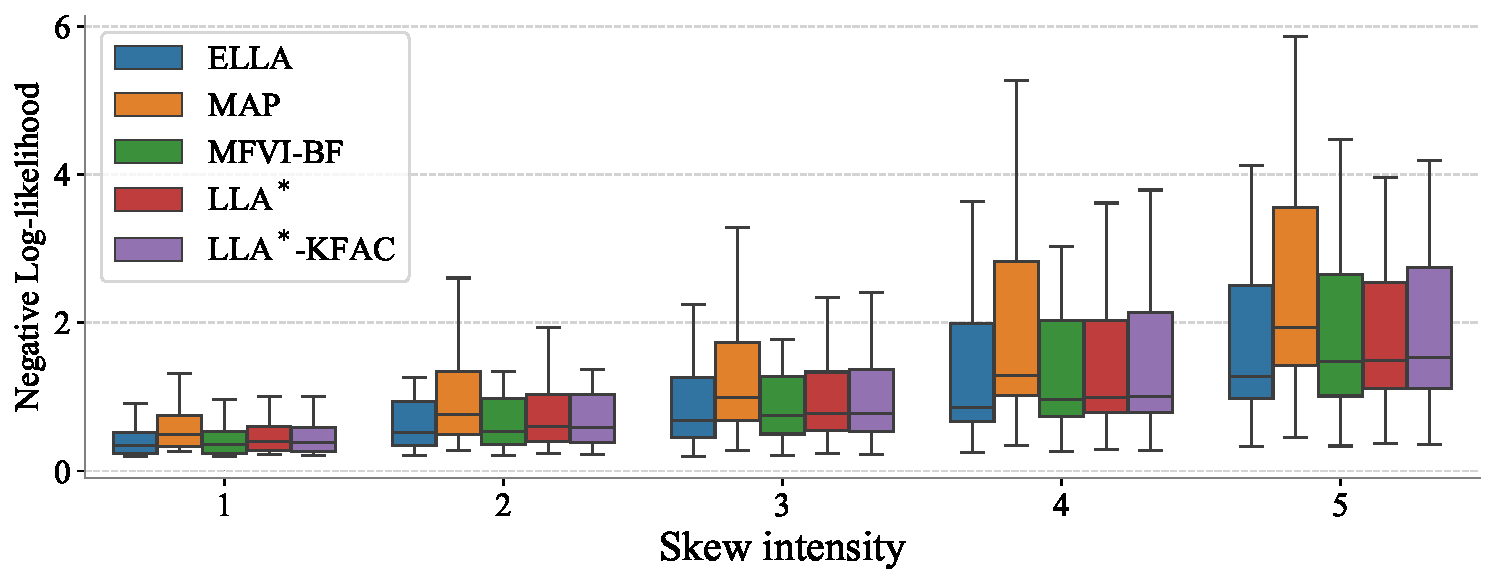
\includegraphics[width=0.9\textwidth]{cifar10_resnet56_corruption_0.pdf}
    \caption{NLL on CIFAR-10 corruptions for models trained with ResNet-56 architecture.}
    \label{fig:corruption0}
\end{figure}
\end{column}
\begin{column}{0.5\textwidth}
\begin{figure}[h]
    \centering
    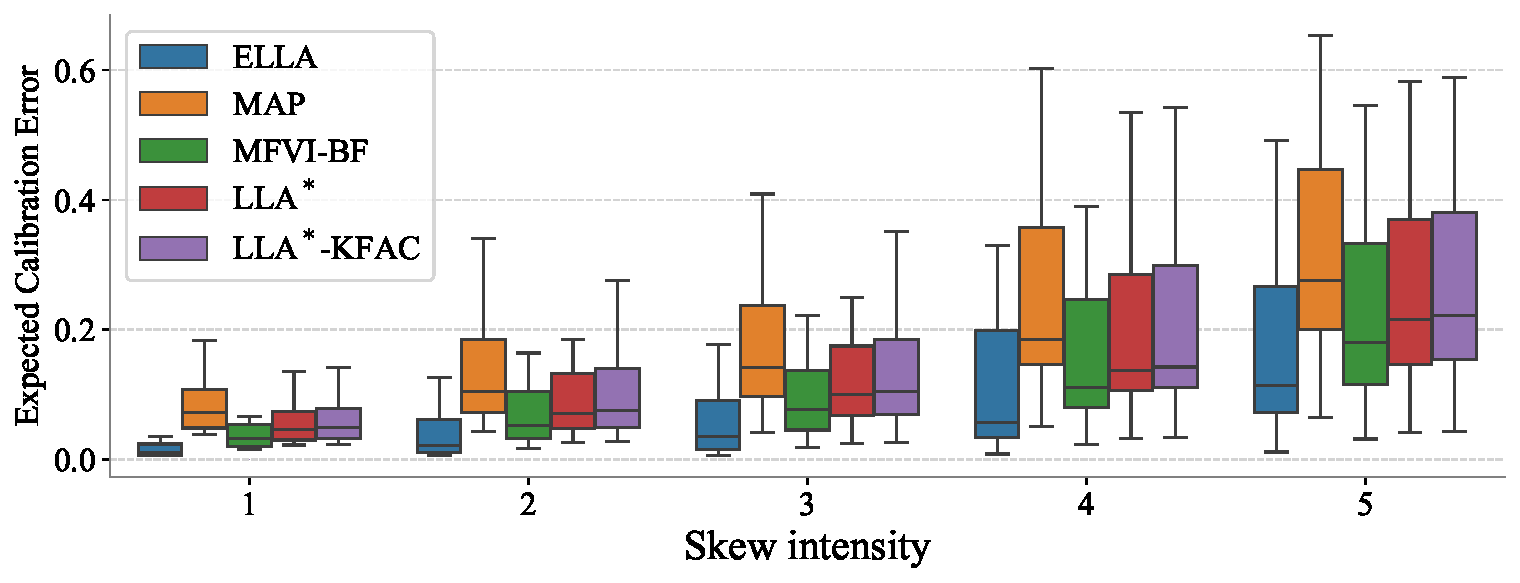
\includegraphics[width=0.9\textwidth]{cifar10_resnet56_corruption_2.pdf}
    \caption{ECE on CIFAR-10 corruptions for models trained with ResNet-56 architecture.}
    \label{fig:corruption2}
\end{figure}
\end{column}
\end{columns}

\end{frame}
\begin{frame}{Experimental Results: Classification}

\begin{columns}
\begin{column}{0.5\textwidth}
\begin{figure}[h]
    \centering
    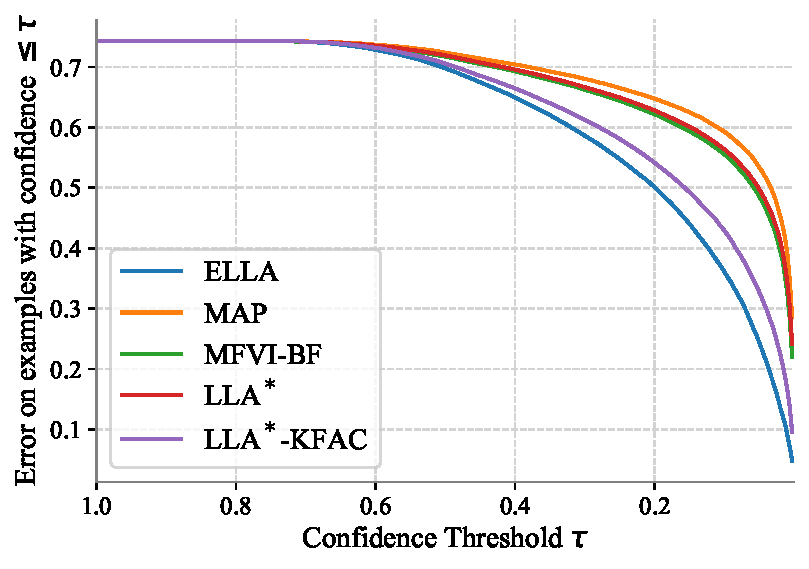
\includegraphics[width=1.0\textwidth]{acc_vs_conf.pdf}
    \caption{Error versus confidence plots for methods trained on CIFAR-10 with ResNet-20 and tested on CIFAR-10+SVHN.}
    \label{fig:corruption0}
\end{figure}
\end{column}
\begin{column}{0.5\textwidth}
\begin{figure}[h]
    \centering
    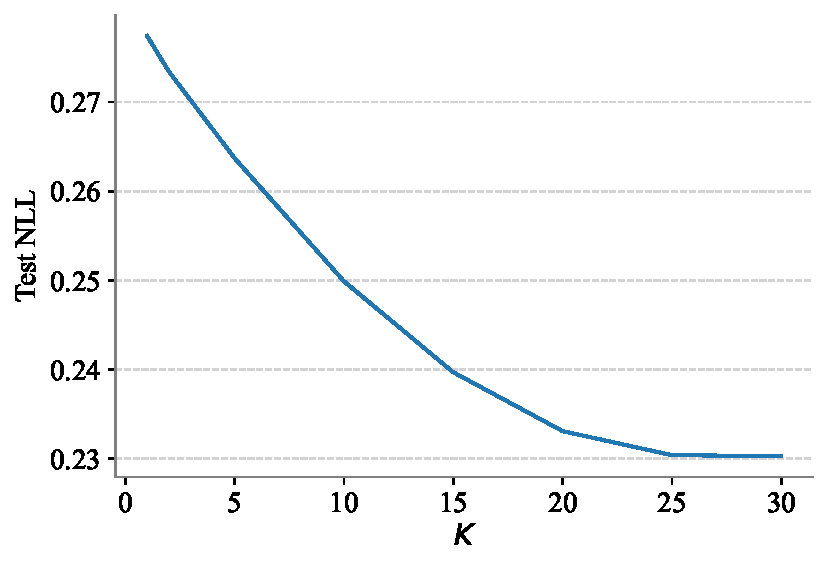
\includegraphics[width=1.0\textwidth]{perf_vs_K.pdf}
    \caption{Test NLL of ELLA varies w.r.t. K on CIFAR-10 with ResNet-20.}
    \label{fig:corruption2}
\end{figure}
\end{column}
\end{columns}


\end{frame}

\begin{frame}{Experimental Results: Classification}
\begin{table}[t]
  \centering
  \footnotesize
  \setlength{\tabcolsep}{5pt}
  \begin{tabular}{
   >{\raggedright\arraybackslash}p{11ex}%
   *{9}{>{\raggedleft\arraybackslash}p{4.5ex}}%
  }
  \toprule
  \multirow{2}{*}[-0.5ex]{\scriptsize Method} & 
  \multicolumn{3}{c}{\scriptsize ResNet-18} & 
  \multicolumn{3}{c}{\scriptsize ResNet-34} & 
  \multicolumn{3}{c}{\scriptsize ResNet-50} \\
  \cmidrule(lr){2-4} \cmidrule(lr){5-7} \cmidrule(lr){8-10}
  & Acc. & NLL & ECE & Acc. & NLL & ECE & Acc. & NLL & ECE \\
  \midrule
  \emph{ELLA}  & 69.8 & 1.243 & \textbf{0.015} & 73.3 & 1.072 & \textbf{0.018} & \textbf{76.2} & 0.948 & \textbf{0.018} \\
  \emph{MAP}   & 69.8 & 1.247 & 0.026 & 73.3 & 1.081 & 0.035 & \textbf{76.2} & 0.962 & 0.037 \\
  \emph{MFVI-BF} & \textbf{70.3} & \textbf{1.218} & 0.042 & \textbf{73.7} & \textbf{1.043} & 0.033 & 76.1 & \textbf{0.945} & 0.030 \\
  \bottomrule
  \end{tabular}
  \caption{Comparison on test accuracy (\%) $\uparrow$, NLL $\downarrow$, and ECE $\downarrow$ on ImageNet. Average over 3 runs.}
  \vskip 0.05in
  \label{table:4}
\end{table}

\begin{table}[h]
  \centering
  \normalsize
  \setlength{\tabcolsep}{5.5pt}
  \begin{tabular}{
   >{\raggedright\arraybackslash}p{6ex}%
   >{\raggedleft\arraybackslash}p{4.5ex}%
   >{\raggedleft\arraybackslash}p{4.5ex}%
   >{\raggedleft\arraybackslash}p{4.5ex}%
  }
  \toprule
  Method & Acc. & NLL & ECE\\
  \midrule
  \emph{ELLA} & 81.6 & 0.695 & 0.022\\
  \emph{MAP} & 81.5 & 0.700 & 0.039\\
  \bottomrule
  \end{tabular}
  \caption{\footnotesize Comparison on test accuracy (\%) $\uparrow$, NLL $\downarrow$, and ECE $\downarrow$ on ImageNet with ViT-B architecture.}
  \label{table:5}
\end{table}

\end{frame}

\begin{frame}{Key Ideas}

\begin{block}{Problem}
\begin{itemize}
    \item Existing methods: computationally expensive or poor quality
\end{itemize}
\end{block}

\begin{block}{ELLA Solution}
\begin{itemize}
    \item Kernel approximation (Nyström) for linearized Laplace
    \item Maintains quality with computational efficiency
\end{itemize}
\end{block}

\begin{block}{Validation}
\begin{itemize}
    \item Strong theoretical guarantees provided
    \item Competitive accuracy with better calibration (lower ECE)
\end{itemize}
\end{block}

\end{frame}




\end{document} 